\documentclass[article]{jss}

% For algorithms
\usepackage{algorithm}
\usepackage{algorithmic}

% As of 2011, we use the hyperref package to produce hyperlinks in the
% resulting PDF.  If this breaks your system, please commend out the
% following usepackage line and replace \usepackage{icml2016} with
% \usepackage[nohyperref]{icml2016} above.
\usepackage{hyperref}
\usepackage{xcolor}
\definecolor{Ckt}{HTML}{E41A1C}
\definecolor{Min}{HTML}{4D4D4D}%grey30
%{B3B3B3}%grey70
\definecolor{MinMore}{HTML}{377EB8}
\definecolor{Data}{HTML}{984EA3}

% Packages hyperref and algorithmic misbehave sometimes.  We can fix
% this with the following command.
%\newcommand{\theHalgorithm}{\arabic{algorithm}}

% Employ the following version of the ``usepackage'' statement for
% submitting the draft version of the paper for review.  This will set
% the note in the first column to ``Under review.  Do not distribute.''
%\usepackage{icml2016} 
\usepackage{fullpage}

% Employ this version of the ``usepackage'' statement after the paper has
% been accepted, when creating the final version.  This will set the
% note in the first column to ``Proceedings of the...''
%\usepackage[accepted]{icml2016}

\usepackage{tikz}
\usetikzlibrary{arrows}
\usepackage{amssymb,amsmath}
\usepackage{natbib}
\usepackage{amsthm}
\newtheorem{proposition}{Proposition}
\newtheorem{lemma}{Lemma}
\newtheorem{theorem}{Theorem}
\newtheorem{definition}{Definition}
\DeclareMathOperator*{\argmin}{arg\,min}
\DeclareMathOperator*{\sign}{sign}
\DeclareMathOperator*{\Lik}{Lik}
\DeclareMathOperator*{\Peaks}{Peaks}
\DeclareMathOperator*{\HotSpots}{HotSpots}
\newcommand{\Cost}{\text{Cost}}
\usepackage{stfloats}
\DeclareMathOperator*{\Diag}{Diag}
\DeclareMathOperator*{\TPR}{TPR}
\DeclareMathOperator*{\Segments}{Segments}
\DeclareMathOperator*{\Changes}{Changes}
\DeclareMathOperator*{\FPR}{FPR}
\DeclareMathOperator*{\argmax}{arg\,max}
\DeclareMathOperator*{\maximize}{maximize}
\DeclareMathOperator*{\minimize}{minimize}
\newcommand{\ZZ}{\mathbb Z}
\newcommand{\NN}{\mathbb N}
\newcommand{\RR}{\mathbb R}


%% -- LaTeX packages and custom commands ---------------------------------------

%% recommended packages
\usepackage{thumbpdf,lmodern}

%% another package (only for this demo article)
\usepackage{framed}

%% new custom commands
\newcommand{\class}[1]{`\code{#1}'}
\newcommand{\fct}[1]{\code{#1()}}


%% -- Article metainformation (author, title, ...) -----------------------------

%% - \author{} with primary affiliation
%% - \Plainauthor{} without affiliations
%% - Separate authors by \And or \AND (in \author) or by comma (in \Plainauthor).
%% - \AND starts a new line, \And does not.
\author{Toby Dylan Hocking\\Northern Arizona University
   \And Guillaume Bourque\\McGill University}
\Plainauthor{Toby Dylan Hocking, Guillaume Bourque}

%% - \title{} in title case
%% - \Plaintitle{} without LaTeX markup (if any)
%% - \Shorttitle{} with LaTeX markup (if any), used as running title
\title{A disk-based functional pruning algorithm for optimal changepoint
  detection in genomic data} 

\Plaintitle{A disk-based functional pruning algorithm for optimal changepoint
  detection in large genomic data} 

%\Shorttitle{A Short Demo Article in \proglang{R}}
\Shorttitle{Disk-based optimal changepoint detection in large data}

%% - \Abstract{} almost as usual
\Abstract{ This article describes a new algorithm and \proglang{R}
  package for optimal changepoint detection in large genomic data
  sets. Previous packages have used in-memory implementations, which
  limit application to relatively small data sets. The proposed
  PeakSegPipeline package implements disk-based storage in order to
  compute optimal changepoint models for the large data sets which are
  widespread in genomics.}

%% - \Keywords{} with LaTeX markup, at least one required
%% - \Plainkeywords{} without LaTeX markup (if necessary)
%% - Should be comma-separated and in sentence case.
\Keywords{Dynamic programming, optimal changepoint detection, peak
  detection, genomic data, \proglang{R}} 

\Plainkeywords{Dynamic programming, optimal changepoint detection, peak
  detection, genomic data, R} 

%% - \Address{} of at least one author
%% - May contain multiple affiliations for each author
%%   (in extra lines, separated by \emph{and}\\).
%% - May contain multiple authors for the same affiliation
%%   (in the same first line, separated by comma).
\Address{
  Toby Dylan Hocking\\
  Northern Arizona University\\
  School of Informatics, Computing, and Cyber Systems\\
  Flagstaff, AZ, USA\\
  E-mail: \email{Toby.Hocking@R-project.org}\\
  %URL: \url{https://eeecon.uibk.ac.at/~zeileis/}
}

\begin{document}


%% -- Introduction -------------------------------------------------------------

%% - In principle "as usual".
%% - But should typically have some discussion of both _software_ and _methods_.
%% - Use \proglang{}, \pkg{}, and \code{} markup throughout the manuscript.
%% - If such markup is in (sub)section titles, a plain text version has to be
%%   added as well.
%% - All software mentioned should be properly \cite-d.
%% - All abbreviations should be introduced.
%% - Unless the expansions of abbreviations are proper names (like "Journal
%%   of Statistical Software" above) they should be in sentence case (like
%%   "generalized linear models" below).

\section[Introduction: optimal changepoint detection in R]{Introduction: optimal changepoint detection in \proglang{R}} \label{sec:intro}

The PeakSegOptimal package provides an in-memory implementation of the
PeakSeg model \citep{Hocking-constrained-changepoint-detection}.

%% -- Manuscript ---------------------------------------------------------------

%% - In principle "as usual" again.
%% - When using equations (e.g., {equation}, {eqnarray}, {align}, etc.
%%   avoid empty lines before and after the equation (which would signal a new
%%   paragraph.
%% - When describing longer chunks of code that are _not_ meant for execution
%%   (e.g., a function synopsis or list of arguments), the environment {Code}
%%   is recommended. Alternatively, a plain {verbatim} can also be used.
%%   (For executed code see the next section.)

\section{Models and software} \label{sec:models}


% \begin{leftbar}
% Note that around the \verb|{equation}| above there should be no spaces (avoided
% in the {\LaTeX} code by \verb|%| lines) so that ``normal'' spacing is used and
% not a new paragraph started.
% \end{leftbar}

% \proglang{R} provides a very flexible implementation of the general GLM
% framework in the function \fct{glm} \citep{Chambers+Hastie:1992} in the
% \pkg{stats} package. Its most important arguments are
% \begin{Code}
% glm(formula, data, subset, na.action, weights, offset,
%   family = gaussian, start = NULL, control = glm.control(...),
%   model = TRUE, y = TRUE, x = FALSE, ...)
% \end{Code}
% where \code{formula} plus \code{data} is the now standard way of specifying
% regression relationships in \proglang{R}/\proglang{S} introduced in
% \cite{Chambers+Hastie:1992}. The remaining arguments in the first line
% (\code{subset}, \code{na.action}, \code{weights}, and \code{offset}) are also
% standard  for setting up formula-based regression models in
% \proglang{R}/\proglang{S}. The arguments in the second line control aspects
% specific to GLMs while the arguments in the last line specify which components
% are returned in the fitted model object (of class \class{glm} which inherits
% from \class{lm}). For further arguments to \fct{glm} (including alternative
% specifications of starting values) see \code{?glm}. For estimating a Poisson
% model \code{family = poisson} has to be specified.

% \begin{leftbar}
% As the synopsis above is a code listing that is not meant to be executed,
% one can use either the dedicated \verb|{Code}| environment or a simple
% \verb|{verbatim}| environment for this. Again, spaces before and after should be
% avoided.

% Finally, there might be a reference to a \verb|{table}| such as
% Table~\ref{tab:overview}. Usually, these are placed at the top of the page
% (\verb|[t!]|), centered (\verb|\centering|), with a caption below the table,
% column headers and captions in sentence style, and if possible avoiding vertical
% lines.
% \end{leftbar}

% \begin{table}[t!]
% \centering
% \begin{tabular}{lllp{7.4cm}}
% \hline
% Type           & Distribution & Method   & Description \\ \hline
% GLM            & Poisson      & ML       & Poisson regression: classical GLM,
%                                            estimated by maximum likelihood (ML) \\
%                &              & Quasi    & ``Quasi-Poisson regression'':
%                                            same mean function, estimated by
%                                            quasi-ML (QML) or equivalently
%                                            generalized estimating equations (GEE),
%                                            inference adjustment via estimated
%                                            dispersion parameter \\
%                &              & Adjusted & ``Adjusted Poisson regression'':
%                                            same mean function, estimated by
%                                            QML/GEE, inference adjustment via
%                                            sandwich covariances\\
%                & NB           & ML       & NB regression: extended GLM,
%                                            estimated by ML including additional
%                                            shape parameter \\ \hline
% Zero-augmented & Poisson      & ML       & Zero-inflated Poisson (ZIP),
%                                            hurdle Poisson \\
%                & NB           & ML       & Zero-inflated NB (ZINB),
%                                            hurdle NB \\ \hline
% \end{tabular}
% \caption{\label{tab:overview} Overview of various count regression models. The
% table is usually placed at the top of the page (\texttt{[t!]}), centered
% (\texttt{centering}), has a caption below the table, column headers and captions
% are in sentence style, and if possible vertical lines should be avoided.}
% \end{table}


%% -- Illustrations ------------------------------------------------------------

%% - Virtually all JSS manuscripts list source code along with the generated
%%   output. The style files provide dedicated environments for this.
%% - In R, the environments {Sinput} and {Soutput} - as produced by Sweave() or
%%   or knitr using the render_sweave() hook - are used (without the need to
%%   load Sweave.sty).
%% - Equivalently, {CodeInput} and {CodeOutput} can be used.
%% - The code input should use "the usual" command prompt in the respective
%%   software system.
%% - For R code, the prompt "R> " should be used with "+  " as the
%%   continuation prompt.
%% - Comments within the code chunks should be avoided - these should be made
%%   within the regular LaTeX text.

\section{Illustrations} \label{sec:illustrations}

For one sample, MACS2 detected one peak, and our PeakSegFPOP algorithm
can be used to find the optimal boundaries of that peak
(Figure~\ref{fig:one-peak}).

For another sample, MACS2 detected five peaks, and our PeakSegFPOP
algorithm can be used to find a more likely model with three peaks
(Figure~\ref{fig:three-peaks}).

% \begin{leftbar}
% For code input and output, the style files provide dedicated environments.
% Either the ``agnostic'' \verb|{CodeInput}| and \verb|{CodeOutput}| can be used
% or, equivalently, the environments \verb|{Sinput}| and \verb|{Soutput}| as
% produced by \fct{Sweave} or \pkg{knitr} when using the \code{render_sweave()}
% hook. Please make sure that all code is properly spaced, e.g., using
% \code{y = a + b * x} and \emph{not} \code{y=a+b*x}. Moreover, code input should
% use ``the usual'' command prompt in the respective software system. For
% \proglang{R} code, the prompt \code{"R> "} should be used with \code{"+  "} as
% the continuation prompt. Generally, comments within the code chunks should be
% avoided -- and made in the regular {\LaTeX} text instead. Finally, empty lines
% before and after code input/output should be avoided (see above).
% \end{leftbar}

\begin{figure}[t!]
\centering

\includegraphics{jss-figure-more-likely-models-one-peak}
\caption{\label{fig:one-peak} Default peak model from the baseline
  MACS2 algorithm (top) and the optimal peak model computed using the
  proposed PeakSegFPOP algorithm (bottom).}
\end{figure}

\begin{figure}[t!]
\centering
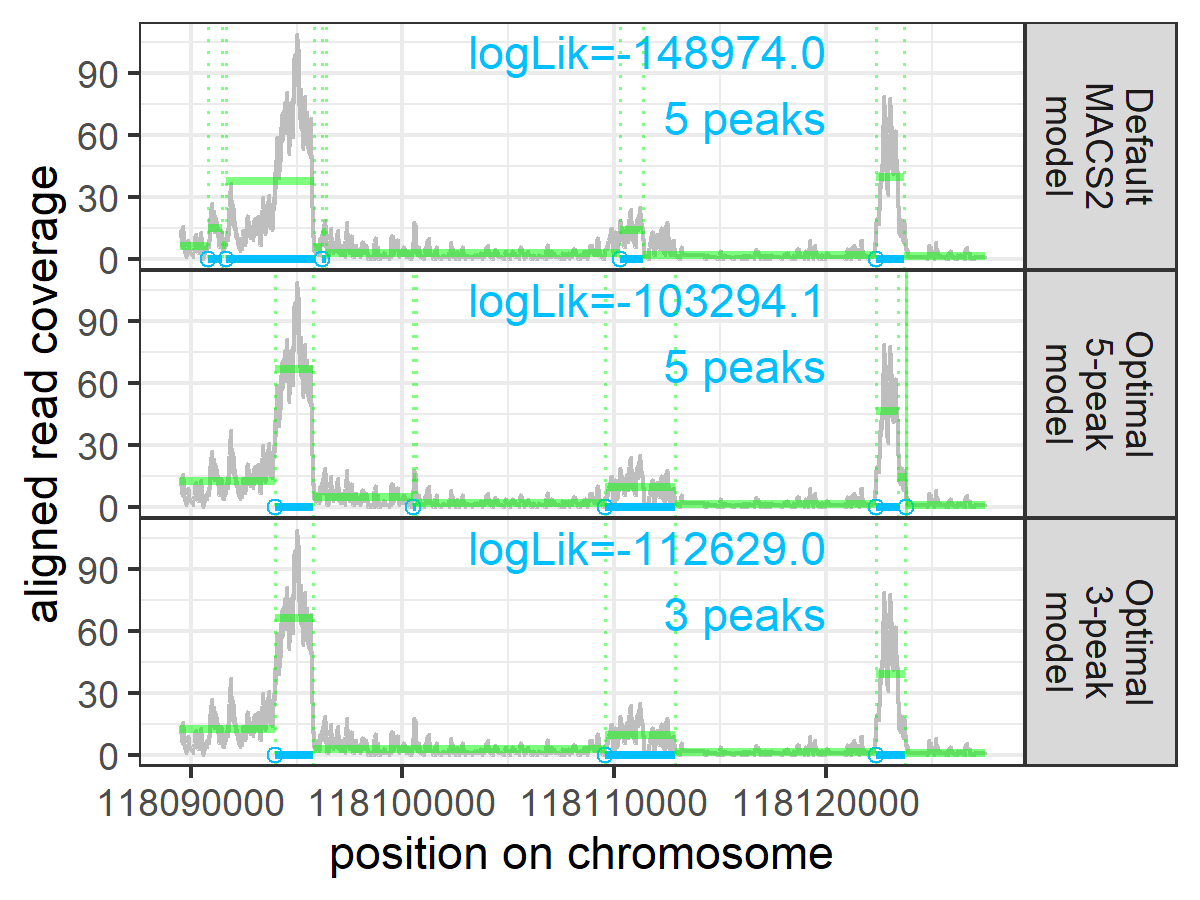
\includegraphics{jss-figure-more-likely-models-three-peaks}
\caption{\label{fig:three-peaks} The peak model from the baseline
  MACS2 algorithm detected five peaks (top), and our PeakSegFPOP
  algorithm can be used to find a more likely model with three peaks
  (bottom).}
\end{figure}
 
% \begin{figure}[t!]
% \centering
% 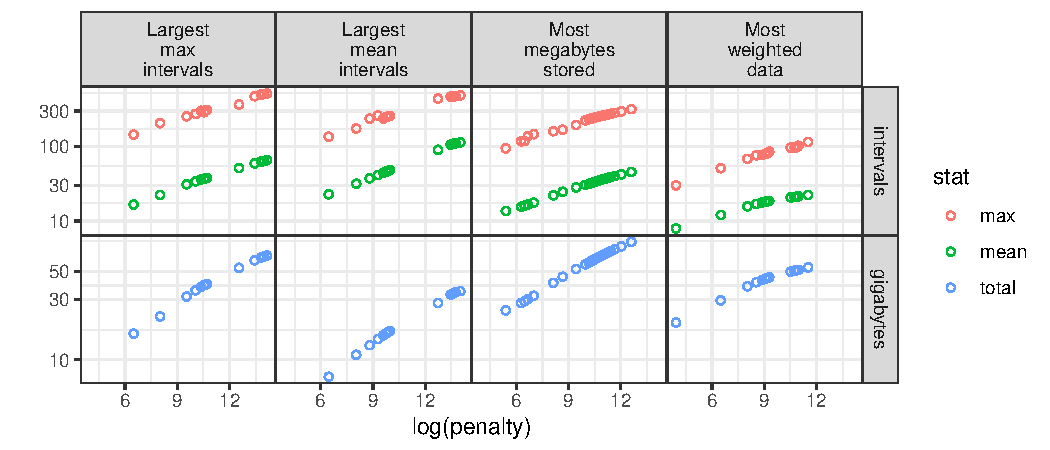
\includegraphics{jss-figure-target-intervals-models-penalty}
% \caption{\label{fig:target-intervals-models-penalty} The PeakSegFPOP
%   algorithm was used to compute optimal models for six of the largest
%   problems (panels from left to right) for a variety of penalty
%   parameters (x-axis). Y-axes show empirical measurements of cost
%   function pieces (intervals, top panel), timings (minutes, middle
%   panel), and disk usage (gigabytes, bottom panel).}
% \end{figure}

\begin{figure}[t!]
\centering
\begin{minipage}{3.1in}
  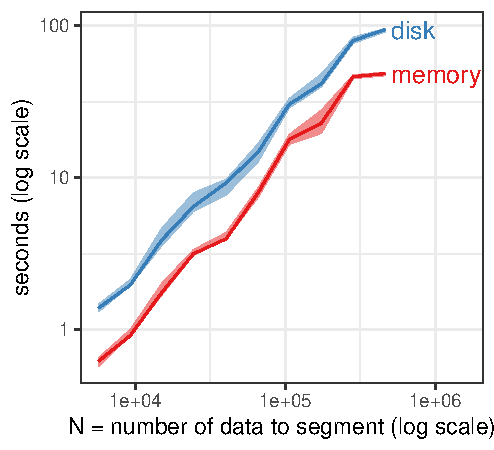
\includegraphics{jss-figure-disk-memory-compare-speed}
\end{minipage} 
\begin{minipage}{3.1in}
  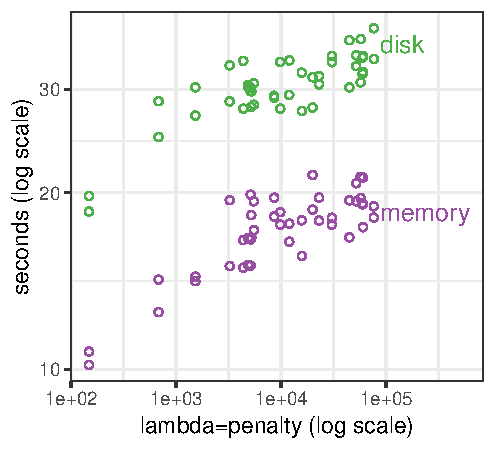
\includegraphics{jss-figure-disk-memory-compare-speed-penalty}
\end{minipage}
\caption{\label{fig:disk-memory-compare-speed} The disk-based
  implementation is only a constant factor slower than the
  memory-based implementation.}
\end{figure}

% \begin{figure}[t!]
% \centering
% 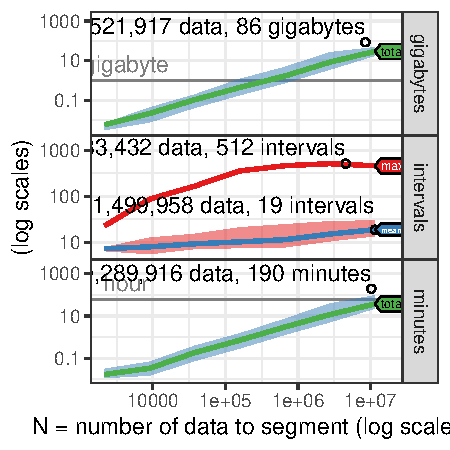
\includegraphics{jss-figure-target-intervals-models-all}
% \caption{\label{fig:target-intervals-models-all} The PeakSegFPOP algorithm
%   was used on the large data sets in the
%   benchmark. Data sizes range from $N=10^2$ to $10^7$ weighted data to
%   segment (x-axis); disk usage (top panel) and computation time
%   (bottom panel) are log-linear $O(N \log N)$.}
% \end{figure}
 
\begin{figure}[t!]
\centering
\begin{minipage}{3.1in}
  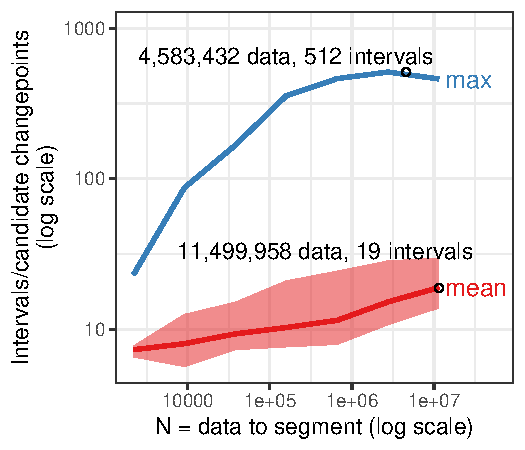
\includegraphics{jss-figure-target-intervals-models}
\end{minipage} 
\begin{minipage}{3.1in}
  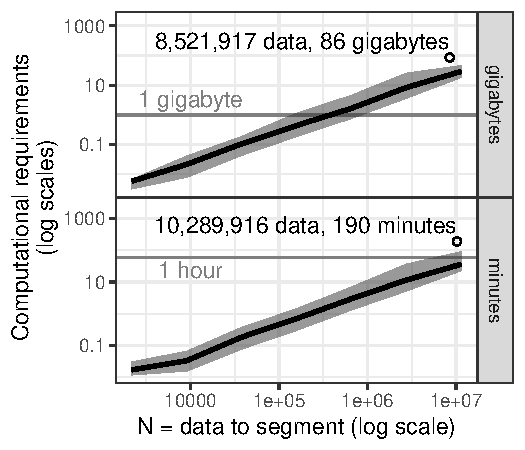
\includegraphics{jss-figure-target-intervals-models-computation}
\end{minipage}
\caption{\label{fig:target-intervals-models-all} The PeakSegFPOP algorithm
  was used on the large data sets in the
  benchmark. Data sizes range from $N=10^2$ to $10^7$ weighted data to
  segment (x-axis); disk usage (top panel) and computation time
  (bottom panel) are log-linear $O(N \log N)$.}
\end{figure}
 
\begin{figure}[t!]
\centering
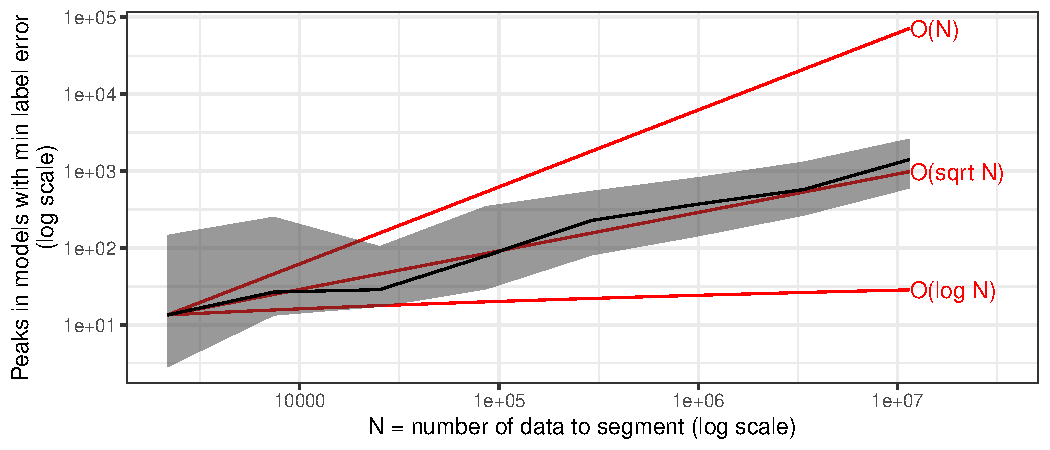
\includegraphics{jss-figure-data-peaks}
\caption{\label{fig:data-peaks} The optimal number of peaks increases
  with data set size.}
\end{figure}
 
\newpage

foo
\newpage

bar
\newpage

\subsection{Penalized version of reduced isotonic regression}

\citet{fpop} proposed the Functional Pruning Optimal Partitioning
(FPOP) algorithm to solve the ``penalized'' or ``optimal
partitioning'' version of the segment neighborhood problem, where the
constraint of $K$ segments is replaced by a non-negative penalty
$\lambda\in\RR_+$ on the number of changes in the objective
function. Rather than computing all models from 1 to $K$ segments (as
in the PDPA), the FPOP algorithm computes the single model with $K$
segments (without computing models from 1 to $K-1$ segments). The same
penalization idea can be applied to models with affine constraints
between adjacent segment means.  The penalized version of the reduced
isotonic regression problem (\ref{eq:reduced}) can be stated as
\begin{align}
  \label{eq:penalized_reduced_isotonic}
  \minimize_{
    \substack{
    \mathbf m\in\RR^n\\
\mathbf c\in\{0,1\}^{n-1}
}
  %\mathbf t\in\{1,\dots,n\}^{K+1}
    } &\ \ 
  \sum_{t=1}^n \ell(y_t, m_t) + \lambda \sum_{t=1}^{n-1} I(c_t \neq 0) \\
  \text{subject to\,} &\ \ c_t = 0 \Rightarrow m_t = m_{t+1}
  \nonumber\\
&\ \ c_t = 1 \Rightarrow m_t \leq m_{t+1}.
\nonumber
\nonumber
\end{align}
Note that the $c_t$ variable is a changepoint indicator.  The same
functional pruning techniques used for the GPDPA can be exploited to
create a solver for this problem. This results in the Generalized
Functional Pruning Optimal Partitioning Algorithm.


Let $\overline C_{\lambda,t}(u)$ be the
penalized cost of the most likely segmentation up to data point $t$,
with last segment mean $u$. The initialization for the first data
point is $\overline C_{\lambda,1}(u) = \ell(y_1, u)$. The dynamic programming update rule
for all data points $t>1$ is
\begin{equation}
  \overline C_{\lambda,t}(u) = \ell(y_t, u) + \min\{
  \overline C_{\lambda,t-1}^\leq(u) + \lambda,\, \overline C_{\lambda,t-1}(u)
  \}.
\end{equation}
The same sub-routines described in Section~\ref{sec:MinLess} can be
used to implement the algorithm below, which solves the penalized
reduced isotonic regression problem
(\ref{eq:penalized_reduced_isotonic}).
\begin{algorithm}[H]
\begin{algorithmic}[1]
\STATE Input: data set $\mathbf y\in\RR^n$, penalty constant $\lambda\geq 0$.
\STATE Output: vectors of optimal segment means $U\in\RR^{n}$ and ends $T\in\{1,\dots,n\}^{n}$
\STATE Compute min $\underline y$ and max $\overline y$ of $\mathbf y$.
\label{line:op-min-max}
\STATE $\overline C_{\lambda,1}\gets \text{OnePiece}(y_1, \underline y, \overline y)$
\STATE for data points $t$ from 2 to $n$: // dynamic programming
\label{line:for-dp-t}
\begin{ALC@g}
  \STATE $\text{min\_prev}\gets \lambda + \text{MinLess}(t-1, \overline C_{\lambda,t-1})$
  \label{line:op-MinLess}
  \STATE $\text{min\_new}\gets \text{MinOfTwo}(\text{min\_prev}, \overline C_{\lambda, t-1})$
  \label{line:op-MinOfTwo}
  \STATE $\overline C_{\lambda,t}\gets \text{min\_new} + \text{OnePiece}(y_t, \underline y, \overline y)$
  \label{line:op-AddNew}
\end{ALC@g}
\STATE $u^*,t',u'\gets \text{ArgMin}(\overline C_{\lambda,n})$ // begin decoding
\label{line:op-ArgMin}
\STATE $i\gets 1;\, U_{i}\gets u^*;\, T_{i}\gets t'$
\label{line:op-store-i}
\STATE while $t' > 0$:
\begin{ALC@g}
  \STATE if $u' < \infty$: $u^*\gets u'$
  \STATE $t',u'\gets\text{FindMean}(u^*, \overline C_{\lambda,t'})$
  \STATE $i\gets i+1;\, U_{i}\gets u^*;\, T_{i}\gets t'$
\label{line:op-i+1}
\end{ALC@g}
\caption{\label{algo:OPIR}Generalized Functional Pruning Optimal
  Partitioning (GFPOP) for penalized reduced isotonic regression}
\end{algorithmic}
\end{algorithm}

Algorithm~\ref{algo:OPIR} begins by computing the min/max
(line~\ref{line:op-min-max}). The main storage
of the algorithm is $\overline C_{\lambda, t}$, which should be
initialized as an array of $n$ empty FunctionPieceList objects. 

The dynamic programming recursion in this algorithm has only one for
loop over data points $t$ (line~\ref{line:for-dp-t}). The penalty
constant $\lambda$ is added to all of the function pieces that result
from MinLess (line~\ref{line:op-MinLess}), before computing MinOfTwo
(line~\ref{line:op-MinOfTwo}). The last step of each dynamic
programming update is to add the cost of the new data point
(line~\ref{line:op-AddNew}).

The decoding process on lines~\ref{line:op-ArgMin}--\ref{line:op-i+1}
is essentially the same as the GPDPA (Algorithm~\ref{algo:GPDPA}). The
last segment mean and second to last segment end are first stored on
line~\ref{line:op-store-i} in $(U_1,T_1)$. For each other segment $i$,
the mean and previous segment end are stored on line~\ref{line:op-i+1}
in $(U_i,T_i)$. Note that there should be space to store $(U_i,T_i)$
parameters for up to $n$ segments. However, there are usually less
than $n$ segments, and the algorithm should return a special flag for
unused parameters, for example $(U_i=\infty, T_i=-1)$.

The time complexity of Algorithm~\ref{algo:OPIR} is $O(n I)$, where
$I$ is the time complexity of the MinLess and MinOfTwo
sub-routines. As in the GPDPA, the time complexity of these
sub-routines is linear in the number of intervals (FunctionPiece
objects) that are used to represent the $\overline C_{\lambda, t}$
cost functions. Since the number of intervals in real data is
typically $I=O(\log n)$ (see Section~\ref{sec:results_time}), the
overall time complexity of Algorithm~\ref{algo:OPIR} is on average
$O(n \log n)$.

\subsection{Generalized Functional Pruning Optimal Partitioning
  Solvers}
\label{sec:GFPOP}

The GFPOP algorithm can solve problems with more general constraints
than reduced isotonic regression. Let $G=(V,E)$ be a directed graph
that represents the model constraints (for examples see
Figure~\ref{fig:state-graphs}). The vertices $V=\{1,\dots,|V|\}$ can be
represented as integers, one for every distinct state. The edges
$E=\{1,\dots,|E|\}$ is another set of integers, each of which represents
one of the possible changes between states. Each edge/change $c\in E$
has corresponding data
$(\underline v_c, \overline v_c, \lambda_c, g_c)$ which specifies a
transition from state $\underline v_c$ to state $\overline v_c$, with
a penalty of $\lambda_c\in\RR_+$, and a constraint function
$g_c:\RR\times\RR\rightarrow\RR$.

\begin{figure*}
  \centering
\parbox{1in}{
\centering \textbf{Unconstrained}\\
  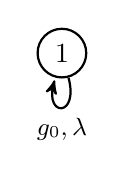
\begin{tikzpicture}[->,>=stealth',shorten >=1pt,auto,node distance=3cm,
                    thick,main node/.style={circle,draw}]

  \node[main node] (1) {1};

  \path[every node/.style={font=\sffamily\small}]
    (1) edge [loop below] node {$g_0, \lambda$} (1);
\end{tikzpicture}
}
\parbox{1in}{
\centering \textbf{Reduced\\
isotonic\\
 regression}\\
  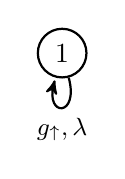
\begin{tikzpicture}[->,>=stealth',shorten >=1pt,auto,node distance=3cm,
                    thick,main node/.style={circle,draw}]

  \node[main node] (1) {1};

  \path[every node/.style={font=\sffamily\small}]
    (1) edge [loop below] node {$g_\uparrow, \lambda$} (1);
\end{tikzpicture}
}
\parbox{1.5in}{
\centering \textbf{Peak detection}
  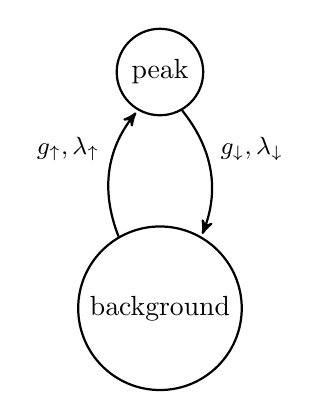
\begin{tikzpicture}[->,>=stealth',shorten >=1pt,auto,node distance=3cm,
                    thick,main node/.style={circle,draw}]

  \node[main node] (1) {peak};
  \node[main node] (2) [below of=1] {background};

  \path[every node/.style={font=\sffamily\small}]
    (2) edge [bend left] node {$g_\uparrow, \lambda_\uparrow$} (1)
    (1) edge [bend left] node {$g_\downarrow, \lambda_\downarrow$} (2);
\end{tikzpicture}
}
\parbox{2.5in}{
\centering \textbf{Unimodal regression}
  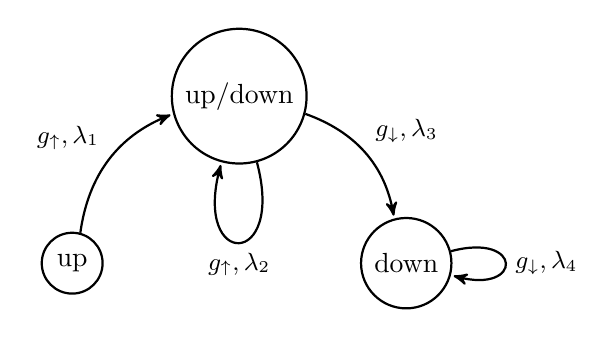
\begin{tikzpicture}[->,>=stealth',shorten >=1pt,auto,node distance=3cm,
                    thick,main node/.style={circle,draw}]

  \node[main node] (1) {up/down};
  \node[main node] (2) [below left of=1] {up};
  \node[main node] (3) [below right of=1] {down};

  \path[every node/.style={font=\sffamily\small}]
    (2) edge [bend left] node {$g_\uparrow, \lambda_1$} (1)
    (1) edge [loop below] node {$g_\uparrow, \lambda_2$} (1)
    (1) edge [bend left] node {$g_\downarrow, \lambda_3$} (3)
    (3) edge [loop right] node {$g_\downarrow, \lambda_4$} (3);
\end{tikzpicture}
}
\caption{Examples of state graphs for four models. Nodes represent
  states and edges represent changes. Each change has a corresponding
  penalty $\lambda$, and a function $g$ that determines what types of
  changes are possible ($g_0$ any change, $g_\uparrow$ non-decreasing,
  $g_\downarrow$ non-increasing). Even if there is no edge from a node
  to itself, it is still possible to stay in the same state without
  introducing a changepoint and penalty. Note that the Unimodal
  regression state X should be interpreted as ``can change X''
  e.g. up/down means ``can change up/down.'' }
  \label{fig:state-graphs}
\end{figure*}
\begin{figure}[H]
  \centering
\parbox{2in}{
\centering
\textbf{Reduced Isotonic Regression}\\
  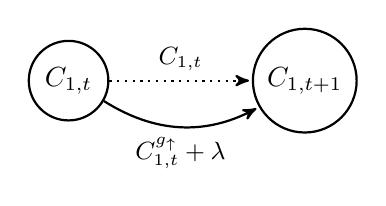
\begin{tikzpicture}[->,>=stealth',shorten >=1pt,auto,node distance=3cm,
  thick,main node/.style={circle,draw}]
  \node[main node] (t) {$C_{1,t}$};
  \node[main node] (t1) [right of=t] {$C_{1, t+1}$};
  \path[every node/.style={font=\small}]
    (t) edge [dotted] node {$C_{1, t}$} (t1)
    (t) edge [black, bend right] node [below] {$C_{1, t}^{g_\uparrow}+\lambda$} (t1)
;
\end{tikzpicture}
}
\parbox{2in}{
\centering
\textbf{Peak detection}\\
  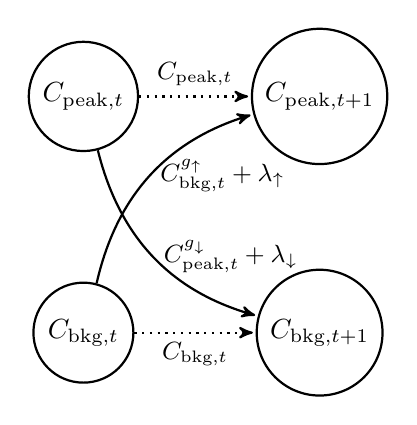
\begin{tikzpicture}[->,>=stealth',shorten >=1pt,auto,node distance=3cm,
  thick,main node/.style={circle,draw}]
  \node[main node] (peak_t) {$C_{\text{peak},t}$};
  \node[main node] (bkg_t) [below of=peak_t] {$C_{\text{bkg}, t}$};
  \node[main node] (peak_t1) [right of=peak_t] {$C_{\text{peak}, t+1}$};
  \node[main node] (bkg_t1) [right of=bkg_t] {$C_{\text{bkg}, t+1}$};
  \path[every node/.style={font=\small}]
    (peak_t) edge [dotted] node {$C_{\text{peak}, t}$} (peak_t1)
    (peak_t) edge [black, bend right] node [right] {$C_{\text{peak}, t}^{g_\downarrow}+\lambda_\downarrow$} (bkg_t1)
    (bkg_t) edge [dotted] node[midway, below] {$C_{\text{bkg}, t}$} (bkg_t1)
    (bkg_t) edge [black, bend left] node[right] {$C_{\text{bkg}, t}^{g_\uparrow}+\lambda_\uparrow$} (peak_t1)
;
\end{tikzpicture}
}
\parbox{2in}{
\centering
\textbf{Unimodal regression}\\
  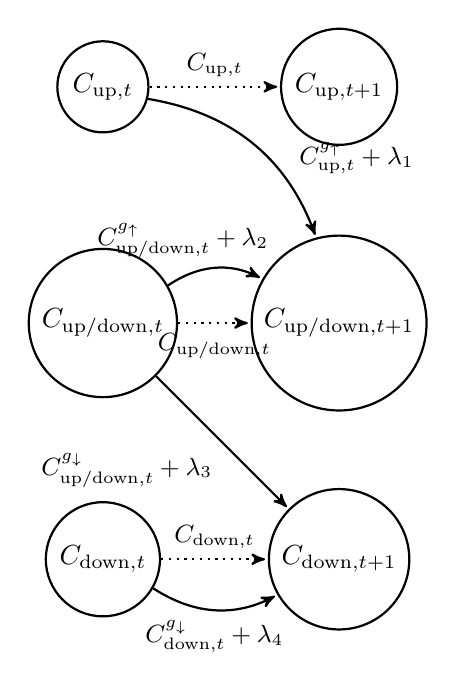
\begin{tikzpicture}[->,>=stealth',shorten >=1pt,auto,node distance=3cm,
  thick,main node/.style={circle,draw}]
  \node[main node] (up_t) {$C_{\text{up},t}$};
  \node[main node] (up_down_t) [below of=up_t] {$C_{\text{up/down}, t}$};
  \node[main node] (down_t) [below of=up_down_t] {$C_{\text{down}, t}$};
  \node[main node] (up_t1) [right of=up_t] {$C_{\text{up}, t+1}$};
  \node[main node] (up_down_t1) [below of=up_t1] {$C_{\text{up/down}, t+1}$};
  \node[main node] (down_t1) [below of=up_down_t1] {$C_{\text{down}, t+1}$};
  \path[every node/.style={font=\small}]
    (up_t) edge [dotted] node {$C_{\text{up}, t}$} (up_t1)
    (up_down_t) edge [dotted] node[midway, below] {$C_{\text{up/down}, t}$} (up_down_t1)
    (down_t) edge [dotted] node {$C_{\text{down}, t}$} (down_t1)
    (up_t) edge [black, bend left] node [near end] {$C_{\text{up}, t}^{g_\uparrow}+\lambda_{1}$} (up_down_t1)
    (up_down_t) edge [black, bend left] node [above] {$C_{\text{up/down}, t}^{g_\uparrow}+\lambda_{2}\hspace{0.8cm}$} (up_down_t1)
    (up_down_t) edge [black] node [below left] {$C_{\text{up/down}, t}^{g_\downarrow}+\lambda_3$} (down_t1)
    (down_t) edge [black, bend right] node [midway, below] {$C_{\text{down}, t}^{g_\downarrow}+\lambda_4$} (down_t1)
;
\end{tikzpicture}
}
\caption{Computation graphs which represent the dynamic programming
  updates (\ref{eq:generalDP}) for the state graph models in
  Figure~\ref{fig:state-graphs}. Nodes represent cost functions
  $C_{s,t}$ in each state $s$ at data $t$ and $t+1$. Edges represent
  inputs to the $\min\{\}$ operation (solid for a changepoint, dotted
  for no change). For example in reduced isotonic regression, $C_{1,t+1}(u) = \ell(y_{t+1}, u) + \min\{ C_{1,t}(u), C_{1,t}^{g_{\uparrow}}(u) + \lambda \}$.
}
  \label{fig:computation-graphs}
\end{figure}

In the optimization problem below we
also allow $c=0$, which implies no penalty $\lambda_0=0$, and means no
change:
\begin{align}
  \label{eq:GFPOP_problem}
  \minimize_{
    \substack{
    \mathbf m\in\RR^n,\ \mathbf s\in V^n\\
\mathbf c\in \{0,1,\dots,|E|\}^{n-1}
}
    } &\ \ 
  \sum_{t=1}^n \ell(y_t, m_t) + \sum_{t=1}^{n-1} \lambda_{c_t} \\
  \text{subject to \hskip 0.9cm} &\ \ c_t = 0 \Rightarrow m_t = m_{t+1}
\text{ and } s_t= s_{t+1}
  \nonumber\\
&\ \ c_t \neq 0 \Rightarrow g_{c_t}(m_t, m_{t+1})\leq 0\text{ and }
(s_t,s_{t+1})=(\underline v_{c_t}, \overline v_{c_t}).
\nonumber
\end{align}
If some states are desired at the start or end, then those constraints
$s_1\in \underline S, s_n\in\overline S$ can also be enforced.  To
compute the solution to this optimization problem, we propose the
following dynamic programming algorithm.

Let $C_{s,t}(u)$ be the optimal cost with mean $u$ and state $s$ at
data point $t$. This quantity can be recursively computed using
dynamic programming. The initialization for the first data point is
$ C_{s,1}(u) = \ell(y_1, u)$ for all states $s$. The dynamic
programming update rule for all data points $t>1$ is
\begin{equation}
\label{eq:generalDP}
   C_{s,t}(u) = \ell(y_t, u) + \min\{
   M_{s,t-1}(u),\,  C_{s,t-1}(u)
  \},
\end{equation}
where the minimum cost of all possible changes to state $s$ from time
point $t-1$ is
\begin{equation}
  M_{s,t-1}(u) = \min_{c\in E_s} C^{g_c}_{\underline v_c, t-1}(u) + \lambda_c,
\end{equation}
and the set of all changes going to state $s$ is
\begin{equation}
  E_s = \{c\in E \mid \overline v_c = s\}.
\end{equation}
The computations required for the dynamic programming updates
(\ref{eq:generalDP}) can be visualized using a computation graph
(Figure~\ref{fig:computation-graphs}).

The pseudocode for the algorithm which implements the dynamic
programming updates (\ref{eq:generalDP}) is stated below.
\begin{algorithm}[H]
\begin{algorithmic}[1]
\STATE Input: data $\mathbf y$ and weights $\mathbf w$ (both size $n$), 
number of vertices/states $|V|$, starts $\underline S\subseteq V$, 
edges/transitions $E$.
\STATE Allocate $|V|\times n$ array of optimal cost functions $C_{s,t}$, 
each initialized to NULL.
\STATE for $t$ from $1$ to $n$:
\begin{ALC@g}
  \STATE if $t==1$:
  \begin{ALC@g}
    \STATE for $s$ in $\underline S$: // initialize cost for all possible starting states
    \begin{ALC@g}
      \STATE $C_{s,t}\gets\text{InitialCost}(y_t, w_t)$
    \end{ALC@g}
  \end{ALC@g}
  \STATE else:
  \begin{ALC@g}
    \STATE for $s$ from $1$ to $|V|$: 
    \begin{ALC@g}
      \STATE if $C_{s,t-1}$ is NOT NULL: // previous cost in this state has been computed
      \begin{ALC@g}
        \STATE $C_{s,t}\gets C_{s,t-1}$ // cost of staying in this state (no change)
      \end{ALC@g}
    \end{ALC@g}
    \STATE for ($\underline v$, $\overline v$, $\lambda$,
    ConstrainedCost) in $E$:
    \begin{ALC@g}
      \STATE if $C_{\underline v,t-1}$ is NOT NULL: // previous cost has been computed
      \begin{ALC@g}
        \STATE
        $\text{cost\_of\_change}\gets
        \text{ConstrainedCost}(C_{\underline v, t-1})$
        \STATE
        $\text{cost\_of\_change.set}
        (\underline v, t-1)$
        \STATE
        $\text{cost\_of\_change.addPenalty}
        (\text{$\lambda$})$
        \STATE if $C_{\overline v,t}$ is NULL:
        \begin{ALC@g}
          \STATE $C_{\overline v,t}\gets\text{cost\_of\_change}$
        \end{ALC@g}
        \STATE else:
        \begin{ALC@g}
          \STATE
          $C_{\overline v,t}\gets \text{MinOfTwo}(C_{\overline v,t},
          \text{cost\_of\_change})$
        \end{ALC@g}
      \end{ALC@g}
    \end{ALC@g}
    \STATE for $s$ from $1$ to $|V|$:
    \begin{ALC@g}
      \STATE if $C_{s,t}$ is NOT NULL:
      \begin{ALC@g}
        \STATE $C_{s,t}\text{.addDataPoint}(y_t, w_t)$
      \end{ALC@g}
    \end{ALC@g}
  \end{ALC@g}
\end{ALC@g}
\STATE Output: $|V|\times n$ array of optimal cost functions $C_{s,t}$.
\caption{\label{algo:GFPOP}Generalized Functional Pruning Optimal
  Partitioning Algorithm, Dynamic Programming (GFPOP-DP)}
\end{algorithmic}
\end{algorithm}

The algorithm above performs several checks if $C_{s,t}$ is NULL or
not (lines 9, 12, 16, 21). All costs are initialized as NULL (line
2). After having performed the cost update for data $t$, a NULL cost
$C_{s,t}$ means that state $s$ is not feasible at data $t$. For each
constraint function $g$ there is a corresponding ConstrainedCost
sub-routine that is mentioned on lines~11 and 13 (e.g. no constraint
$g_0$ MinUnconstrained, non-decreasing change $g_\uparrow$ MinLess,
non-increasing change $g_\downarrow$ MinMore). 

The average time and space complexity of Algorithm~\ref{algo:GFPOP} is
$O(|V| n I)$ where $|V|$ is the number of states and $I$ is the
average number of of intervals stored in the $|V|\times n$ array of
$C_{s,t}$ cost functions. We observed that $I=\log n$ in the empirical
tests of the peak detection model on ChIP-seq data
(Section~\ref{sec:results_time}), so we expect that the average time
complexity of Algorithm~\ref{algo:GFPOP} is $O(|V| n\log n)$.

Note that the algorithm above only performs the dynamic
programming. The decoding of optimal model parameters is achieved
using the algorithm below.

\begin{algorithm}[H]
\begin{algorithmic}[1]
\STATE Output: $|V|\times n$ array of optimal cost functions $C_{s,t}$, 
ends $\overline S\subseteq V$.
\STATE Allocate
$\mathbf m\in\RR^n$ (mean), 
$\mathbf s\in\ZZ^n$ (state), 
$\mathbf t\in\ZZ^n$ (segment end).
\STATE $u^*,s^*,t',s'\gets \text{ArgMin}(C_{\cdot,n}, \overline S)$ // begin decoding
\STATE $i\gets 1;\, m_{i}\gets u^*;\, s_i\gets s^*;\, t_{i}\gets n$
\STATE while $t' > 0$:
\begin{ALC@g}
  \STATE $i\gets i+1;\, t_{i}\gets t'$
  \STATE $u^*,s^*,t',s'\gets \text{ArgMin}(C_{s',t'})$
  \STATE $m_{i}\gets u^*;\, s_i\gets s^*$
\end{ALC@g}
\STATE Output: 
$\mathbf m$, 
$\mathbf s$, 
$\mathbf t$.
\caption{\label{algo:GFPOP-decode}Generalized Functional Pruning Optimal
  Partitioning Algorithm, decoding (GFPOP-decode)}
\end{algorithmic}
\end{algorithm}


 

% \begin{CodeChunk}
% \begin{CodeInput}
% R> m_pois <- glm(Days ~ (Eth + Sex + Age + Lrn)^2, data = quine,
% +    family = poisson)
% \end{CodeInput}
% \end{CodeChunk}
% %
% To account for potential overdispersion we also consider a negative binomial
% GLM.
% %
% \begin{CodeChunk}
% \begin{CodeInput}
% R> library("MASS")
% R> m_nbin <- glm.nb(Days ~ (Eth + Sex + Age + Lrn)^2, data = quine)
% \end{CodeInput}
% \end{CodeChunk}
% %
% In a comparison with the BIC the latter model is clearly preferred.
% %
% \begin{CodeChunk}
% \begin{CodeInput}
% R> BIC(m_pois, m_nbin)
% \end{CodeInput}
% \begin{CodeOutput}
%        df      BIC
% m_pois 18 2046.851
% m_nbin 19 1157.235
% \end{CodeOutput}
% \end{CodeChunk}
% %
% Hence, the full summary of that model is shown below.
% %
% \begin{CodeChunk}
% \begin{CodeInput}
% R> summary(m_nbin)
% \end{CodeInput}
% \begin{CodeOutput}
% Call:
% glm.nb(formula = Days ~ (Eth + Sex + Age + Lrn)^2, data = quine, 
%     init.theta = 1.60364105, link = log)

% Deviance Residuals: 
%     Min       1Q   Median       3Q      Max  
% -3.0857  -0.8306  -0.2620   0.4282   2.0898  

% Coefficients: (1 not defined because of singularities)
%             Estimate Std. Error z value Pr(>|z|)    
% (Intercept)  3.00155    0.33709   8.904  < 2e-16 ***
% EthN        -0.24591    0.39135  -0.628  0.52977    
% SexM        -0.77181    0.38021  -2.030  0.04236 *  
% AgeF1       -0.02546    0.41615  -0.061  0.95121    
% AgeF2       -0.54884    0.54393  -1.009  0.31296    
% AgeF3       -0.25735    0.40558  -0.635  0.52574    
% LrnSL        0.38919    0.48421   0.804  0.42153    
% EthN:SexM    0.36240    0.29430   1.231  0.21818    
% EthN:AgeF1  -0.70000    0.43646  -1.604  0.10876    
% EthN:AgeF2  -1.23283    0.42962  -2.870  0.00411 ** 
% EthN:AgeF3   0.04721    0.44883   0.105  0.91622    
% EthN:LrnSL   0.06847    0.34040   0.201  0.84059    
% SexM:AgeF1   0.02257    0.47360   0.048  0.96198    
% SexM:AgeF2   1.55330    0.51325   3.026  0.00247 ** 
% SexM:AgeF3   1.25227    0.45539   2.750  0.00596 ** 
% SexM:LrnSL   0.07187    0.40805   0.176  0.86019    
% AgeF1:LrnSL -0.43101    0.47948  -0.899  0.36870    
% AgeF2:LrnSL  0.52074    0.48567   1.072  0.28363    
% AgeF3:LrnSL       NA         NA      NA       NA    
% ---
% Signif. codes:  0 '***' 0.001 '**' 0.01 '*' 0.05 '.' 0.1 ' ' 1

% (Dispersion parameter for Negative Binomial(1.6036) family taken to be 1)

%     Null deviance: 235.23  on 145  degrees of freedom
% Residual deviance: 167.53  on 128  degrees of freedom
% AIC: 1100.5

% Number of Fisher Scoring iterations: 1


%               Theta:  1.604 
%           Std. Err.:  0.214 

%  2 x log-likelihood:  -1062.546 
% \end{CodeOutput}
% \end{CodeChunk}



%% -- Summary/conclusions/discussion -------------------------------------------

\section{Summary and discussion} \label{sec:summary}


%% -- Optional special unnumbered sections -------------------------------------

\section*{Computational details}

% \begin{leftbar}
% If necessary or useful, information about certain computational details
% such as version numbers, operating systems, or compilers could be included
% in an unnumbered section. Also, auxiliary packages (say, for visualizations,
% maps, tables, \dots) that are not cited in the main text can be credited here.
% \end{leftbar}

% The results in this paper were obtained using
% \proglang{R}~3.4.1 with the
% \pkg{MASS}~7.3.47 package. \proglang{R} itself
% and all packages used are available from the Comprehensive
% \proglang{R} Archive Network (CRAN) at
% \url{https://CRAN.R-project.org/}.


\section*{Acknowledgments}

% \begin{leftbar}
% All acknowledgments (note the AE spelling) should be collected in this
% unnumbered section before the references. It may contain the usual information
% about funding and feedback from colleagues/reviewers/etc. Furthermore,
% information such as relative contributions of the authors may be added here
% (if any).
% \end{leftbar}


%% -- Bibliography -------------------------------------------------------------
%% - References need to be provided in a .bib BibTeX database.
%% - All references should be made with \cite, \citet, \citep, \citealp etc.
%%   (and never hard-coded). See the FAQ for details.
%% - JSS-specific markup (\proglang, \pkg, \code) should be used in the .bib.
%% - Titles in the .bib should be in title case.
%% - DOIs should be included where available.

\bibliography{jss-refs}


% %% -- Appendix (if any) --------------------------------------------------------
% %% - After the bibliography with page break.
% %% - With proper section titles and _not_ just "Appendix".

% \newpage

% \begin{appendix}

% \section{More technical details} \label{app:technical}

% \begin{leftbar}
% Appendices can be included after the bibliography (with a page break). Each
% section within the appendix should have a proper section title (rather than
% just \emph{Appendix}).

% For more technical style details, please check out JSS's style FAQ at
% \url{https://www.jstatsoft.org/pages/view/style#frequently-asked-questions}
% which includes the following topics:
% \begin{itemize}
%   \item Title vs.\ sentence case.
%   \item Graphics formatting.
%   \item Naming conventions.
%   \item Turning JSS manuscripts into \proglang{R} package vignettes.
%   \item Trouble shooting.
%   \item Many other potentially helpful details\dots
% \end{itemize}
% \end{leftbar}


% \section[Using BibTeX]{Using \textsc{Bib}{\TeX}} \label{app:bibtex}

% \begin{leftbar}
% References need to be provided in a \textsc{Bib}{\TeX} file (\code{.bib}). All
% references should be made with \verb|\cite|, \verb|\citet|, \verb|\citep|,
% \verb|\citealp| etc.\ (and never hard-coded). This commands yield different
% formats of author-year citations and allow to include additional details (e.g.,
% pages, chapters, \dots) in brackets. In case you are not familiar with these
% commands see the JSS style FAQ for details.

% Cleaning up \textsc{Bib}{\TeX} files is a somewhat tedious task -- especially
% when acquiring the entries automatically from mixed online sources. However,
% it is important that informations are complete and presented in a consistent
% style to avoid confusions. JSS requires the following format.
% \begin{itemize}
%   \item JSS-specific markup (\verb|\proglang|, \verb|\pkg|, \verb|\code|) should
%     be used in the references.
%   \item Titles should be in title case.
%   \item Journal titles should not be abbreviated and in title case.
%   \item DOIs should be included where available.
%   \item Software should be properly cited as well. For \proglang{R} packages
%     \code{citation("pkgname")} typically provides a good starting point.
% \end{itemize}
% \end{leftbar}

% \end{appendix}

% %% -----------------------------------------------------------------------------


\end{document}
